\documentclass[12pt]{article}

\usepackage[letterpaper, margin=1in]{geometry}
\usepackage{times}
\usepackage{setspace}
\usepackage{lipsum}
\usepackage{graphicx}
\usepackage{float}

\title{Transfer Learning for American Sign Language Dataset}
\author{Josh Hills - 101142996\\COMP 4107\\Professor Holden}
\date{\today}

\begin{document}
\maketitle
\newpage
\subsection*{Introduction}
\quad
Transfer learning is a machine learning technique that allows a pre-trained neural network model to be fine-tuned on a smaller, task-specific dataset. The use of transfer learning has become 
increasingly prevalent in the field of deep learning, specifically in image recognition, natural language processing, and reinforcement learning. The purpose of this final project is to investigate
the effectiveness of transfer learning when applied to the task of classifying ASL hand gestures. There is an abundance of great research studying transfer learning, such as Weiss et al. (2016). We will
build on these foundational studies and surveys to learn how transfer learning can be applied to our specific problem. Transfer learning has lots of potential for reducing computation required in
deep learning projects, making time for computation a topic of this study. The primary goal of this paper is to evaluate the effectiveness of transfer learning, comparing the performance of the fine-tuned
pre-trained models from a model we make without transfer learning. I find transfer learning particularly interesting as an individual, sometimes we feel limited to projects we can do alone because of the 
limited amount of data an individual can collect, computation power an individual has access to. Using transfer learning we can leverage research of others and in a literal sense 
open up the number of possibilities that your average person has in research and development. 

\subsection*{Methods}
\quad
For the training of the model, convolutional neural networks (CNNs) will be used. While we will be testing multiple pre-trained neural networks, we will only be talking about the architecture of VGG16, and how
it is modified to solve our new task. First lets talk about how image classification works. Pretending that image classification is a black box for a second, the task of image classification is given
an input image x, and outputs a single class that the image most likely falls into. For example, if we consider a model trained on the popular ImageNet dataset, given an image the model tries to guess which of the
1000 classes the image most likely is. Enter the VGG16 model for the ImageNet dataset. \\
\begin{figure}[H]
    \centering
    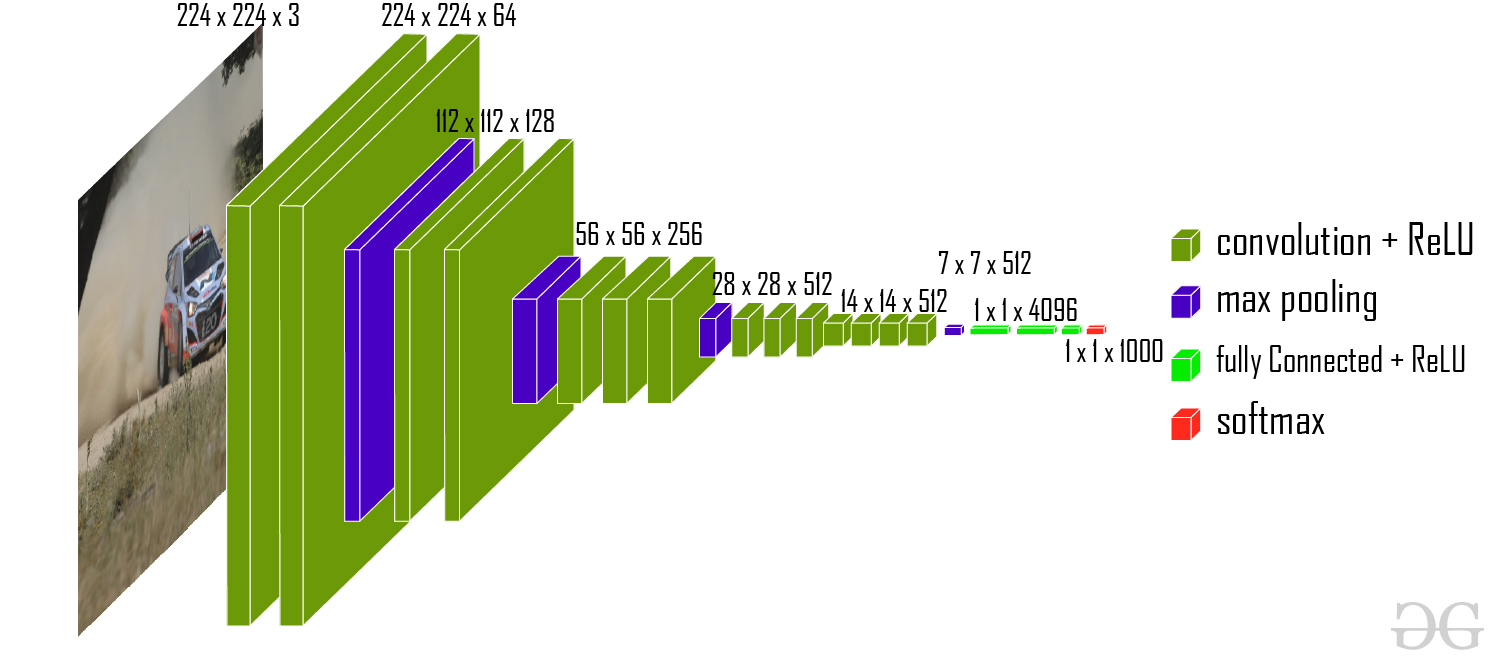
\includegraphics[scale=0.25]{images/vgg-architechture.jpg}\\
    https://www.geeksforgeeks.org/vgg-16-cnn-model/
\end{figure}
The above shows the network architecture of the VGG16 model which was trained using the ImageNet dataset. This dataset contains 224x224 images with RGB channels, this gives us an input tensor of 224x224x3.
As this is an example of a CNN, we then see a series of convolution layers using a ReLU activation followed by max pooling layers. This architecture shows 5 convolution/pooling operations, in some cases there are 2 convolutions before 
pooling and sometimes 3 convolutions. After this series of operations we have a 7x7x512 feature map. Then, this output is flattened to make it a 1x25088 feature vector. Following this is 3 
fully connected layers, finally giving us a 1x1000 output. Using the softmax, we get the class predicted for our image. We can imagine the final output vector as $\hat{y} = [\hat{y_0}; \hat{y_1}; \hat{y_2}; ... ; \hat{y_{999}}]$, which contains scores
of each class, taking the $softmax(\hat{y})$ gives us the probability of each class. The max of the softmax is the predicted class. So why is this useful to us? How can we use this model to predict
the classes for the ASL dataset? Essentially, the reason this is so useful, as I mentioned above, we create a feature map before our actual classification. The features in this map can be useful for a new model. ImageNet has a load of classes [2], we can assume by VGG16's very high accuracy that it has a good understanding of the natural world, and thus maybe understands what a hand looks like, meaning 
where a hand is in the image is not a feature that our fine-tuned model will have to learn. Compared to a model that we train from scratch, will have to use it's limited dataset to figure out more simple features. We cut off
the flattening and then dense layers at the end of the neural network and create our own, we then fit the model using the ASL images and are given a new model. \\


This study uses two main datasets, one directly and one indirectly. While we do not actually use the dataset the ImageNet dataset, I think it is still important to explain it here to gain a full grasp of 
transfer learning's value. ImageNet is a dataset consisting of approximately 14 million images that each belong to one of 1000 classes [3]. ImageNet was first created to establish a good benchmark test
to be used for object categorization. Researchers work hard to develop new and better algorithms to organize and annotate video and image data, better tools require better data to train their algorithms on.
We can imagine how a model build using ImageNet can be used to categorize our pictures, think about this as the technology that allows us to search all the pictures on our iPhones for those containing a cat. 
The second dataset used is ASL Alphabet Test, found on Kaggle. This dataset contains 870 images, each of which contain a hand making the shape of an ASL letter (with some variation). There are
twenty-nine possible classes, these include all the letters A-Z as well as "del", "space", and "nothing". This gives us a total of 30 images per class, with a total of 29 classes providing 870 images.
Nine random images were selected and are displayed below, above them shows their respective classes.\\
\includegraphics*[scale=0.25]{images/example_from_dataset.JPG} \\

This data was split into three subsets: 609 images for training, 174 images for validation, 87 images for test, a 70:20:10 split.
This split ensures that our model is trained and validated using different sets of data, allowing us to evaluate its generalization
performance on unseen images. These splits are also important for another reason, data augmentation.\\


With such a limited dataset, data augmentation is quite useful. Through data augmentation we are able to create a more robust model that 
is accustomed to more variable data. Data augmentation is a technique that applies random transformations to the images, in this case:
flipping, rotating, zooming, adjusting contrast and random translation. These transformations allow us to artificially expand the training dataset. 
To break down these transformations a bit more descriptively:
\begin{itemize}
    \item Random horizontal flipping
    \item Random rotation within a range of ±20\% of the original angle
    \item Random zoom, with a zoom range of ±20\% along both the horizontal and vertical axes
    \item Random contrast adjustment, with a contrast range of ±20\%
    \item Random translation, with a translation range of ±20\% along both the horizontal and vertical axes
\end{itemize}

By incorporating the data augmentation layer into our fine-tuning process, we aimed to increase the models' ability to 
generalize to unseen data, improving the accuracy on the test dataset by approximately 21\%. \\


Now to get into the training of the model. We used the VGG16 model as our based model, pre-trained on the ImageNet dataset as mentioned above. 
We added a custom prediction layer with the number of outputs equal to the number of classes in our dataset (29) and a softmax
activation function for multi-class classification. The final model included the following layers:\\
\includegraphics*[scale=0.4]{images/model_plot.png}\\
\begin{itemize}
    \item \textbf{input\_4:} Input layer, this represents the image with dimensions 200x200 with 3 channels (RGB)
    \item \textbf{vgg16:} VGG16 base model (without the top classification layer)
    \item \textbf{flatten\_1:} Flatten layer to convert the feature maps into a 1D tensor
    \item \textbf{dropout\_1:} Dropout layer with a rate of 0.2 to regularize the model and prevent overfitting
    \item \textbf{dense\_1:} Dense layer (prediction layer) with 29 output units and a softmax activation function
\end{itemize}

The model was then compiled using the Adam optimizer with a learning rate of 0.001 and the sparse categorical cross-entropy loss function.
To quickly explain the Adam (Adaptive Moment Estimation) optimizer, it adapts the learning rate for each weight in the model individually, making 
it more efficient and effective for deep neural networks. It computes adaptive learning rates for each parameter using the first and second moments (the mean and centered variance) of the gradients.
These are estimated with exponential moving averages. The primary benefits of Adam are faster convergence, improved handling of sparse gradients, and 
robustness to noisy data. Sparse categorical cross-entropy loss is used for multi-class classification tasks where the target variable consists of 
integer class labels rather than one-hot-encoded vectors. It computes the cross-entropy loss between the predicted class probabilities and the true class labels.
This is useful when working with lots of classes, as it avoids the need for one-hot encoding the target labels, in this case with 29 classes we could've gotten away with encoding though.
The models' performance was evaluated based on its accuracy during training. The model was trained for 25 epochs, using the training dataset and validating its performance on the validation set.

\section*{Results}
After training our fine-tuned model for 25 epochs, we evaluated its performance on the test dataset.
The model is able to achieve an accuracy of \%69 on the test dataset, which is actually quite impressive considering our small amount of 30
images per class and our high amount of classes at 29. It demonstrated a great ability to generalize to unseen data.
The results indicate that our model understands and classifies the 29 classes in the dataset with a decent accuracy.\\
\includegraphics*[scale=0.5]{images/loss+acc.png}\\
First to address this model, we can see that it finishes with a training accuracy of \%82 and a validation accuracy of \%70, it takes my computer about 28 minutes to train
this model. This far exceeds the time that it would take to train a model that does not use transfer learning. \\
\includegraphics*[scale=0.5]{images/confusion matrix.png}\\
This confusion matrix helps us understand how well our model performed on the test dataset, and gives us some ideas how we could improve it.
For instance, the model is too often predicting class 26 (the "del" symbol), this could be due to an abundance of those characters in the training set, or maybe it is just easily confused about that character 
specifically, this could all be researched in a deeper look into this specific use case. Overall though, we can see that the model does a good job 
at predicting the actual label, this can be seen by looking at the diagonal of the confusion matrix. Now, let's talk about poorer models to make transfer learning look better.\\

To show the effectiveness of 
transfer learning, we also trained a model without using it. This model performed horribly with a testing accuracy of \%6. This is a CNN using the Keras Sequential API, I do not want to spend too much time on the 
architecture as the performance is abysmal.
\begin{itemize}
    \item A 2D convolutional layer with 32 filters, kernel size of (3, 3), ReLU activation, and input shape of (200, 200, 3)
    \item A 2D max-pooling layer with pool size of (2, 2)
    \item A 2D convolutional layer with 64 filters, kernel size of (3, 3), and ReLU activation
    \item A 2D max-pooling layer with pool size of (2, 2)
    \item A 2D convolutional layer with 128 filters, kernel size of (3, 3), and ReLU activation
    \item A 2D max-pooling layer with pool size of (2, 2)
    \item A 2D convolutional layer with 128 filters, kernel size of (3, 3), and ReLU activation
    \item A 2D max-pooling layer with pool size of (2, 2)
    \item A flatten layer to convert the feature maps into a 1D tensor
    \item A dropout layer with a rate of 0.5 to regularize the model and prevent overfitting
    \item A dense layer with 512 units and ReLU activation
    \item A dense layer (output layer) with num\_classes output units and a softmax activation function for multi-class classification
\end{itemize} 
This custom CNN was then compiled using the Adam optimizer, sparse categorical cross-entropy loss function and was evaluated on accuracy (all the same as our TF model).
It trained for 25 epochs and had the same training/validation/testing datasets as the fine-tuned VGG16 model.\\
\includegraphics*[scale=0.5]{images/loss+acc no tf.png}\\
As we can by see the accuracy really learned nothing, and performs not much better than just guessing classes. Through this we can understand the value transfer leaning brings.
\\

Before ending this paper, we trained one more model to see the comparison of results, we will take a look at a model who is trained without the use of data augmentation. As a reminder,
data augmentation is a technique used to artificially expand the training dataset by applying random transformations. To take a look at model used without this critical feature of our model, we trained it identically as 
to the fine-tuned VGG16 model, except we left out the data augmentation layer.\\
\includegraphics*[scale=0.5]{images/loss+acc no aug.png}\\
Through the technique of data augmention, we are able to increase the by \%21. That is going from a test accuracy of \%49 to \%69. It is interesting to note that the training accuracy of the two models are the same, it seems that data augmentation just reduces overfitting.

\section*{Conclusion}
In this paper, we have investigated the effectiveness of transfer learning using a fine-tuned VGG16 model for the classification of ASL images. We have also compared its performance with a custom CNN architecture that does not rely on transfer learning. Our experiments demonstrated that the fine-tuned VGG16 model achieved satisfactory accuracy on the test dataset, outperforming the baseline custom CNN model.\\

The use of transfer learning, data augmentation, and effective preprocessing techniques played a significant role in improving the model's performance. While the obtained accuracy is promising, there is still room for further improvement by fine-tuning hyperparameters, exploring alternative model architectures, and employing larger datasets.\\

In conclusion, our study showcases the potential of transfer learning using pre-trained neural networks for challenging classification tasks, such as ASL image recognition. This research also highlights the importance of data augmentation and proper preprocessing techniques in achieving better generalization to new, unseen data. By building upon these findings, future research can continue to advance the state of the art in ASL recognition and other similar applications.\\


% [2] https://deeplearning.cms.waikato.ac.nz/user-guide/class-maps/IMAGENET/
% [3] https://www.image-net.org/about.php
% [4] https://www.kaggle.com/code/abdul390/asl-recognition-with-convolutional-neural-networks
\end{document}